Considerando le critiche elencate in precedenza e il target d'utenza rilevato si
presenta la seguente proposta di progetto, la quale costituirà la base per
un'eventuale applicazione conforme alle principali norme e linee guida
riguardanti l'usabilità.

\subsection{Architettura dell'informazione}
Per la realizzazione del progetto si è utilizzato un approccio goal-oriented, top down.
Tramite questo approccio il sistema viene rifinito in modo progressivo a partire dagli
obiettivi inizialmente individuati.\\
Il progetto utilizza le linee guida e le interfacce base conformi al moderno
standard \emph{Material design}\cite{MaterialDesign}. Tale linguaggio di design si basa su una semplice
metafora: lo schermo bidimensionale viene pensato come tridimensionale, con oggetti
che hanno una posizione spaziale anche sul terzo asse, in modo da emulare una superficie
che possa creare e muovere volumi. Vi è poi un uso costante di animazioni a supporto di tale metafora e che
aiutano l'utente a individuare l'effetto delle proprie azioni.
Un altro aspetto importante del linguaggio è la semplicità
delle icone e dei widget: se negli anni passati si è assistito ad un enorme
successo delle interfacce
scheumorfiche\footnote{un interfaccia si dice skeumorfica se emula l'estetica di un oggetto reale},
soprattutto grazie all'influenza di IOS nelle interfacce per sistemi mobili,
oggi si assiste ad un ritorno a schermate più semplici, che non utilizzano
così estensivamente metafore di oggetti reali.
Per quanto riguarda le funzionalità, si è scelto di implementare
molte funzioni ausiliarie, ma completamente integrate nel processo
culinario, il quale fa da padrone per l'intero utilizzo dell'applicazione.\\
La ricerca di ricette, siano esse nuove o già parzialmente conosciute, è una
parte molto importante nello sviluppo di un applicazione di supporto alla
cucina. Per questo motivo è stata implementata una soluzione molto potente, rendendo
possibile all'utente combinazioni complesse di filtraggio dei dati.\\
Considerando il requisito riguardante la possibilità di silenziare le notifiche
dell'app stessa, si è progettato il sistema per funzionare in modalità ``non
disturbare''
nel caso in cui il device sia rivolto verso il basso.  Tale funzionalità è
comunque disattivabile dalle opzioni dell'applicazione.

\subsection{Design dell'interazione}

\subsubsection{Blueprint}
Le funzionalità principali sono state suddivise nelle principali macro-aree
funzionali dell'applicazione.  Ciascuna di esse contiene le schermate
relative alle iterazioni ad essa afferenti.  In figura \ref{fig:blueprint}
è riportato il blueprint relativo alle interazioni possibili ed alla struttura
di navigazione dell'applicazione.
\begin{figure}[H]
	\centering
	\caption{Blueprint delle interazioni tra finestre}
	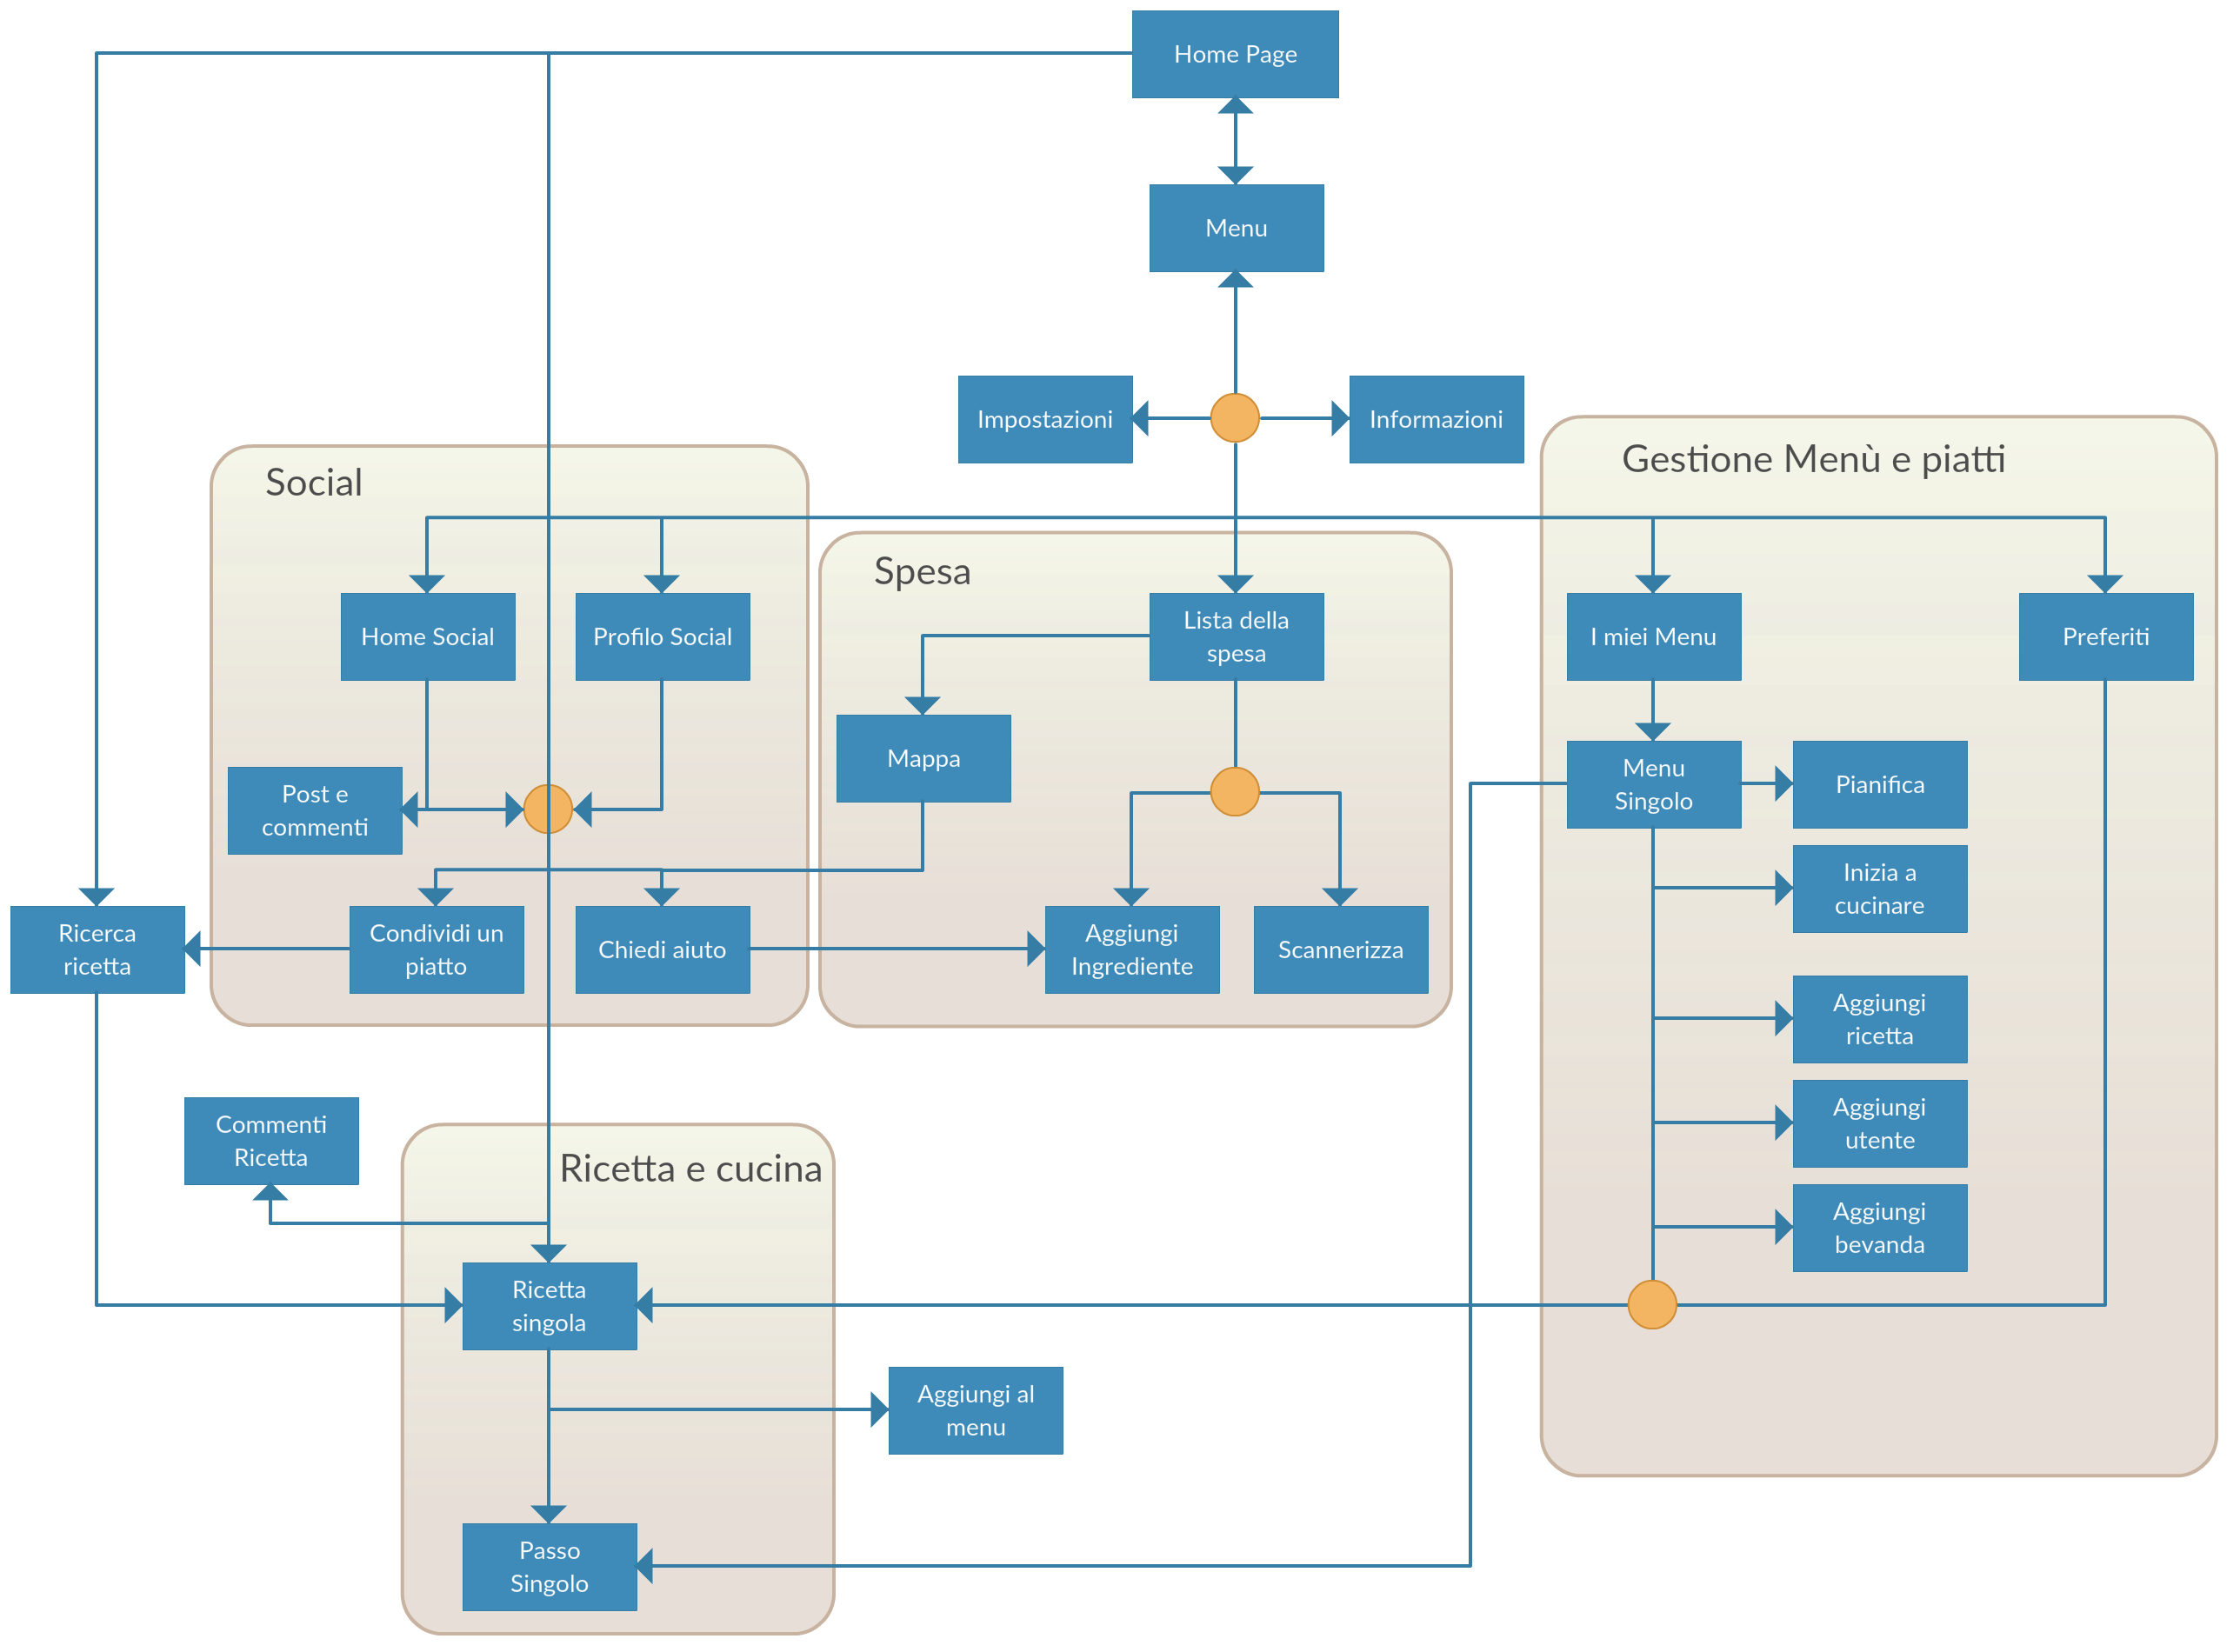
\includegraphics[width=\textwidth]{img/ipc_blueprint}
	\label{fig:blueprint}
\end{figure}
Vi sono anche anche interazioni non specificate nel blueprint poiché troppo
specifiche:
\begin{itemize}
	\item Premendo il tasto ``indietro" si passa alla
	schermata precedente, e così a ritroso fino alla schermata Home.
	Premendo nuovamente il tasto indietro nella pagina principale
	verrà chiusa l'applicazione.
	\item Alcune notifiche contestuali presenti nell'applicazione non
	vengono indicate nel blueprint.
	\item La ricerca è considerata come contestuale, nell'area social
	verranno cercati gli utenti, mentre nelle altre aree verranno cercati i
	singoli piatti (rimandando alla schermata di ricerca avanzata)
	o gli ingredienti.
	\item È possibile modificare la dimensione del testo con gesti \emph{pinch to
	zoom}, la barra presente nelle impostazioni reagirà di conseguenza.
\end{itemize}

\subsubsection{Comandi vocali}
\begin{figure}[H]
	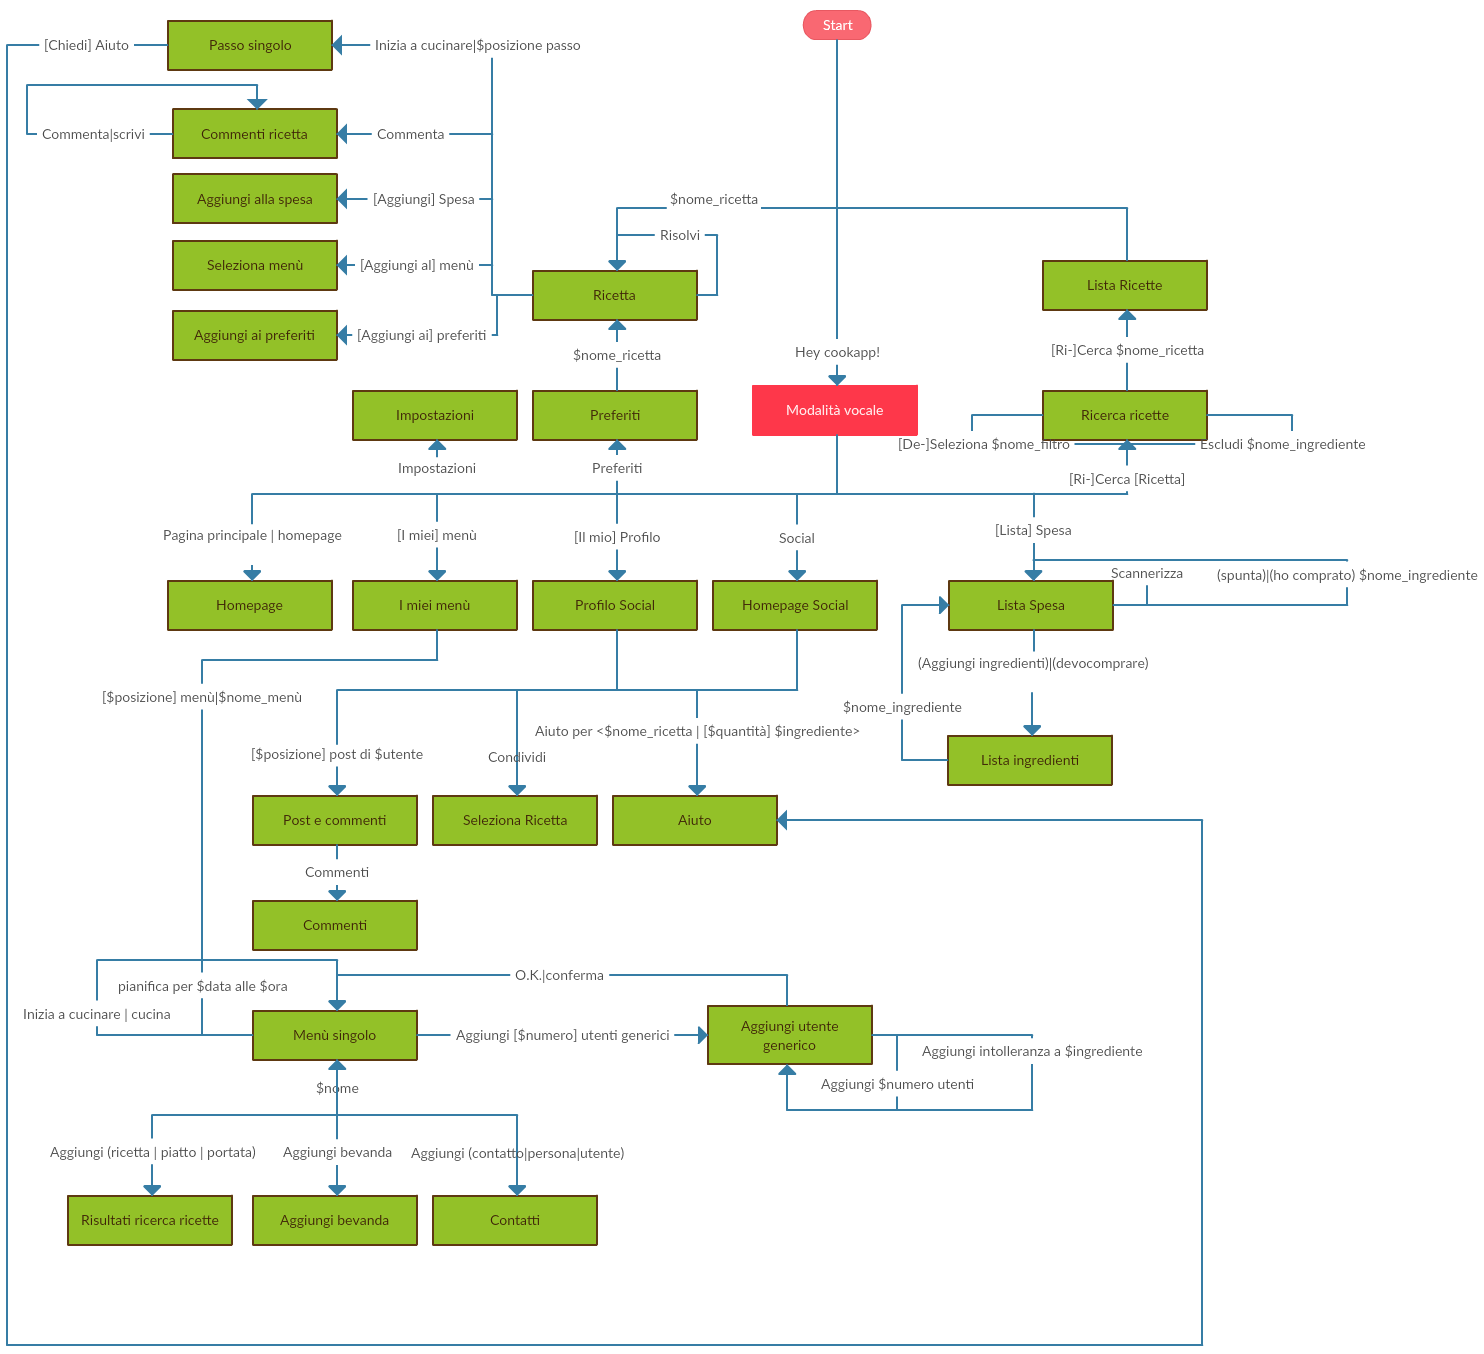
\includegraphics[width=\textwidth]{img/ipc_interazione_audio}
	\caption{schema relativo alle interazioni vocali in linguaggio naturale}
	\label{fig:ipcvocali}
\end{figure}
Sono stati implementati diversi comandi vocali.  L'interazione viene avviata
pronunciando ``hey cookapp!''.  Il sistema di comandi vocali è in grado di
comprendere diverse frasi espresse in linguaggio naturale.  Delle quali si riporta
la lista dei comandi in figura \ref{fig:ipcvocali}.\\
Dalla suddetta interfaccia è possibile invocare diversi comandi per navigare
all'interno dell'applicazione, in modo simile a quanto avviene tramite il menù
di navigazione.  Ogni comando vocale viene poi interpretato contestualmente al compito e alla
schermata in cui viene invocato; in questo modo è possibile eseguire anche task complessi
utilizzando solamente l'interazione vocale.

\subsubsection{Wireframe}

\begin{quote}
 \textbf{Homepage}
\end{quote}
Il punto di partenza dell'interazione con l'applicazione è la home
page (figura \ref{fig:homepage_tooltip}). Tale pagina
si pone l'obiettivo di aiutare l'utente nella scoperta di nuove ricette e, durante
i primi utilizzi, delle funzionalità fondamentali. Si compone di una griglia di ricette
consigliate all'utente in base alle sue preferenze.
Dalla home page è possibile accedere alla ricerca ed al menù di navigazione, in modo da consentire
un rapido accesso alle funzionalità principali già dall'avvio.

\begin{quote}
 \textbf{Menù di navigazione}
\end{quote}
Il menù di navigazione (figura \ref{fig:menu_nav}), in modo analogo a quanto avviene in molte applicazioni che utilizzano material design,
è costituto da un pannello sovrapposto rispetto alle schermate sottostanti e che può venire invocato tramite
un tasto menù o uno swipe dall'estremo sinistro dello schermo. Il menù consente l'accesso ai preferiti, all'elenco dei
menù dell'utente, all'area social, alle impostazioni ed alla lista della spesa, nonché alla pagina iniziale. È infine
possibile accedere al proprio profilo tramite il proprio avatar.

\begin{quote}
 \textbf{Ricerca ricette}
\end{quote}
La ricerca delle ricette (figura \ref{fig:cerca_ricetta}) fornisce un potente pannello che consente di applicare vari filtri.
È infatti possibile escludere ingredienti dalle ricette, selezionare solo alcune portate fra antipasti, primi,
secondi, dolci e piatti unici. È infine possibile cercare ricette di una certa categoria (vegetariane, senza glutine, etc).

\begin{quote}
 \textbf{Area Social}
\end{quote}
L'area social (figura \ref{fig:homepage_social}) contiene le funzionalità relative all'interazione fra gli utenti. L'account viene
mutuato da un famoso social network, dal quale si può modificare il proprio profilo.
È possibile condividere ricette, richiedere aiuto per ingredienti mancanti e passi
della ricetta. Gli utenti possono poi commentare i post che vengono
pubblicati (figura \ref{fig:commenti_social}).

\begin{quote}
 \textbf{Gestione dei Menù}
\end{quote}
L'applicazione utilizza il concetto di menù (figura \ref{fig:menu_tooltip}) per consentire l'organizzazione dei pasti, gestendo gli 
invitati e la pianificazione temporale. Da tale sezione è possibile iniziare a cucinare: in questa modalità vengono
mostrati i passi completati e quelli mancanti per ciascuna ricetta selezionata. Aggiungendo utenti che sono presenti
Aggiungendo ai partecipanti utenti allergici, viene mostrato un avviso per
ciascuna ricetta contenente l'allergene (figure \ref{fig:risolvi_allergia}).  È poi possibile sostiuire la ricetta o
l'allergene.

\begin{quote}
 \textbf{Lista della spesa}
\end{quote}
Tramite la lista della spesa (figura \ref{fig:lista_della_spesa}) è possibile
spuntare gli elementi che si sono già acquistati, richiedere direzioni verso
negozi e supermercati (figure \ref{fig:indicazioni_stradali} e
\ref{fig:indicazioni_stradali_negozi_chiusi}),
utilizzare NFC o fotografare il codice a barre per
selezionare ciò che si è acquistato. È inoltre possibile richiedere aiuto agli amici
tramite il social per gli ingredienti mancanti.

\begin{quote}
 \textbf{Modalità cucina}
\end{quote}
Nella modalità cucina i menù mostrano il progresso della ricetta, ed un tocco
sulle singole ricette conduce al passo corrente. I singoli step
contengono immagini e video contestuali. È scelta del redattore se utilizzare in primo piano un'immagine o un video.
È disponibile un timer nel caso di operazioni che richiedano ad esempio
una cottura o un periodo di attesa. Ciascun passo può essere condiviso sul social per richiedere consigli o aiuto.

\begin{quote}
 \textbf{Impostazioni}
\end{quote}
La schermata delle impostazioni (figura \ref{fig:impostazioni}) permette di modificare la dimensione del testo,
gestire le notifiche e la modalità ``non disturbare''. Tale modalità permette
di disabilitare l'audio e le notifiche, in modo da evitare fastidi all'utente.
È inoltre possibile attivare questa modalità rivolgendo il telefono verso il basso.

\begin{quote}
 \textbf{Notifica contestuale}
\end{quote}
Durante il normale utilizzo del programma vi è la possibilità che appaiano sullo schermo degli aiuti contestuali da parte dell'applicazione.
Lo scopo di tali notifiche è quello di ridurre il carico cognitivo dell'utente, aiutandolo a ricordarsi di alcuni eventi in modo appropriato.
Tali notifiche sono di vari tipi: 
\begin{itemize}
 \item nel caso di menù già pianificati viene ricordato all'utente di iniziare a
	 cucinare all'avvicinarsi del pasto pianificato;
 \item se si deve effettuare la spesa viene mostrato un ingrediente ancora non acquistato;
 \item vengono notificate le richieste di aiuto degli amici;
 \item nella schermata relativa al menù vengono mostrati piatti e bevande consigliati;
 \item se si sta cucinando, viene mostrato il prossimo passo da eseguire.
\end{itemize}
Le notifiche appaiono nella porzione bassa dello schermo durante l'esecuzione,
mentre sono trasmesse al sistema operativo nel caso l'applicazione
sia inattiva.  Tramite un tocco sulle notifiche si viene condotti alla pagina
appropriata. È infine possibile effettuare uno swipe per nasconderle.
